\documentclass{article}
\usepackage[school,simplified]{pgf-umlcd}
\usetikzlibrary{calc}
\usetikzlibrary{positioning}
\usepackage{fullpage}
\usepackage{fancyhdr}
\pagestyle{fancy}
\lhead{}
\rhead{}
\chead{}
\rfoot{\thepage}
\lfoot{Martin Baumgaertner - Tous droits résérvés}
\cfoot{}
\renewcommand{\headrulewidth}{0pt}
\begin{document}  

 
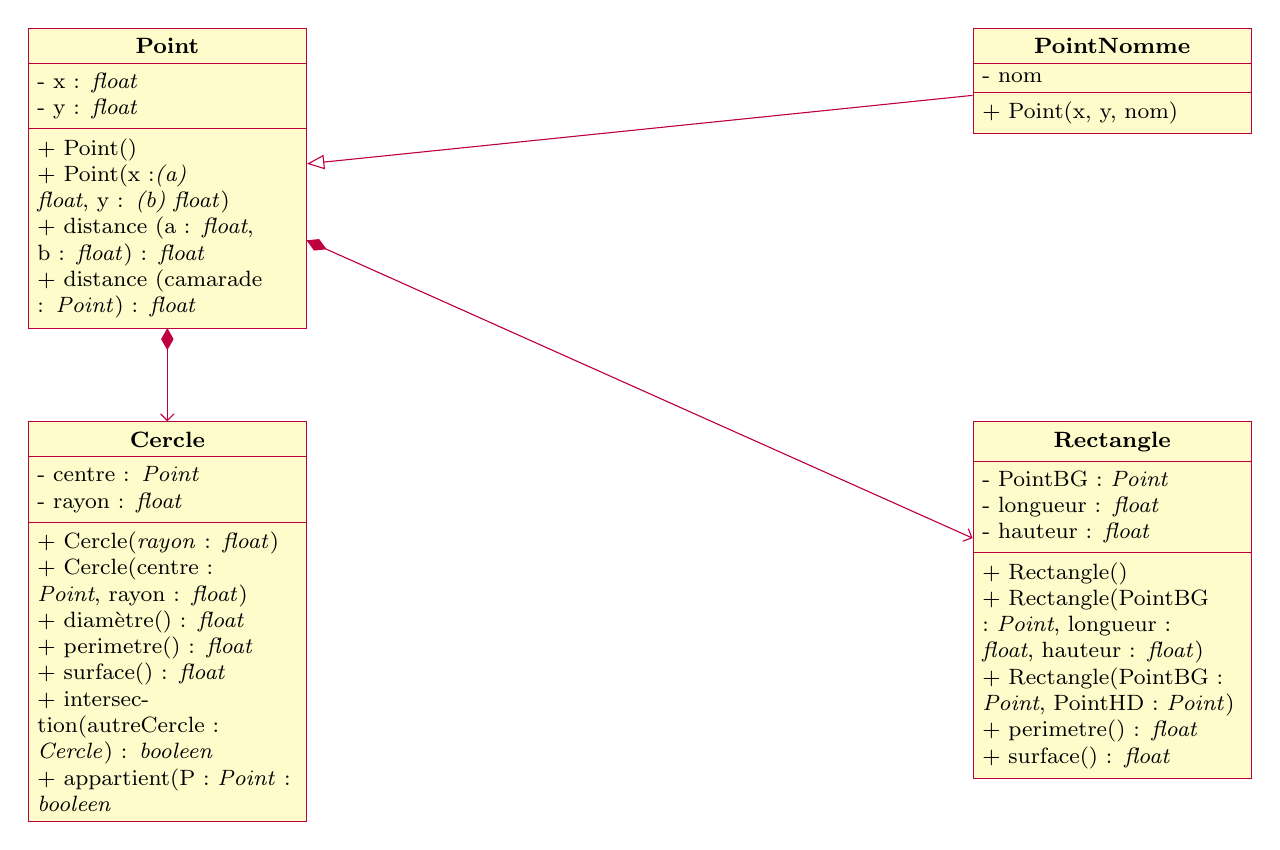
\begin{tikzpicture}[font=\footnotesize] 



\begin{class}[text width = 3.3cm, yshift=-5mm]{Point}{0,5}
    \attribute{- x : \textit{float}}
    \attribute{- y : \textit{float}}
    \operation{+ Point()}
    \operation{+ Point(x :\textit{(a) float}, y : \textit{(b) float})}
    \operation{+ distance (a : \textit{float}, b : \textit{float}) : \textit{float}}
    \operation{+ distance (camarade : \textit{Point}) : \textit{float}}
\end{class}

\begin{class}[text width = 3.3cm, yshift=-5mm]{Cercle}{0,0}
    \attribute{- centre : \textit{Point}}
    \attribute{- rayon : \textit{float}}
    \operation{+ Cercle(\textit{rayon} : \textit{float})}
    \operation{+ Cercle(centre : \textit{Point}, rayon : \textit{float})}
    \operation{+ diamètre() : \textit{float}}
    \operation{+ perimetre() : \textit{float}}
    \operation{+ surface() : \textit{float}}
    \operation{+ intersection(autreCercle : \textit{Cercle}) : \textit{booleen}}
    \operation{+ appartient(P : \textit{Point} : \textit{booleen}}
\end{class}


\begin{class}[text width = 3.3cm, yshift=-5mm]{PointNomme}{12,5}
    \inherit{Point}
    \attribute{- nom}
    \operation{+ Point(x, y, nom)}

\end{class}

\begin{class}[text width = 3.3cm, yshift=-5mm]{Rectangle}{12,0}
    \attribute{- PointBG : \textit{Point}}
    \attribute{- longueur : \textit{float}}
    \attribute{- hauteur : \textit{float}}
    \operation{+ Rectangle()}
    \operation{+ Rectangle(PointBG : \textit{Point}, longueur : \textit{float}, hauteur : \textit{float})}
    \operation{+ Rectangle(PointBG : \textit{Point}, PointHD : \textit{Point})}
    \operation{+ perimetre() : \textit{float}}
    \operation{+ surface() : \textit{float}}
\end{class}

\composition{Point}{}{}{Cercle}
\composition{Point}{}{}{Rectangle}

\end{tikzpicture}
\end{document}